\documentclass[12pt]{article}

\usepackage{amssymb,amsmath,amsfonts,eurosym,geometry,ulem,graphicx,caption,color,setspace,sectsty,comment,footmisc,caption,natbib,pdflscape,subfigure,array,float}

\usepackage[colorlinks = true,
            linkcolor = blue,
            urlcolor  = blue,
            citecolor = black,
            anchorcolor = blue]{hyperref}

\normalem

\onehalfspacing
\newtheorem{theorem}{Theorem}
\newtheorem{corollary}[theorem]{Corollary}
\newtheorem{proposition}{Proposition}
\newenvironment{proof}[1][Proof]{\noindent\textbf{#1.} }{\ \rule{0.5em}{0.5em}}

\newtheorem{hyp}{Hypothesis}
\newtheorem{subhyp}{Hypothesis}[hyp]
\renewcommand{\thesubhyp}{\thehyp\alph{subhyp}}

\newcommand{\red}[1]{{\color{red} #1}}
\newcommand{\blue}[1]{{\color{blue} #1}}

\newcolumntype{L}[1]{>{\raggedright\let\newline\\arraybackslash\hspace{0pt}}m{#1}}
\newcolumntype{C}[1]{>{\centering\let\newline\\arraybackslash\hspace{0pt}}m{#1}}
\newcolumntype{R}[1]{>{\raggedleft\let\newline\\arraybackslash\hspace{0pt}}m{#1}}

\geometry{left=1.0in,right=1.0in,top=1.0in,bottom=1.0in}

\begin{document}

\begin{titlepage}
\title{Community Currencies as Crisis Response: Results from a Randomized Control Trial in Kenya\thanks{Working draft}}
\author{Rebecca Mqamelo\thanks{Minerva Schools at KGI, \href{mailto:rebecca.mqamelo@minerva.kgi.edu}{rebecca.mqamelo@minerva.kgi.edu}}}
\date{May 2021}
\maketitle
\begin{abstract}
\noindent In 2020, Grassroots Economics’ \textit{Community Inclusion Currency} (CIC) model was adopted by the Kenya Red Cross as a humanitarian response to the Covid-19 pandemic. This paper presents the results of what may be the world’s first randomized control trial in this area. Unlike most cash transfer programs, recipients are sent cryptocurrencies rather than cash or mobile money, enabling an unprecedented level of impact evaluation. Results show that CIC transfers of \$30 are associated with \$93.51 increase in beneficiaries' wallet balance, a \$23.17 increase in monthly income, a \$16.30 increase in monthly spending, a \$6.31 increase in average trade size and a \$28.43 increase in expenditure on food and water. However, the difference in treatment effects for males versus females suggests gender imbalances persist. This study serves as an important prototype for cash transfer models that keep money flowing locally and support bottom-up economic resilience.\\
\vspace{0in}\\
\noindent\textbf{Keywords:} community inclusion currency, complementary currency, unconditional cash transfer, randomized control trial, blockchain, humanitarian response, Covid-19, Kenya\\
%\vspace{0in}\\
%\noindent\textbf{JEL Codes:} key1, key2, key3\\

\bigskip
\end{abstract}
\setcounter{page}{0}
\thispagestyle{empty}
\end{titlepage}
\pagebreak \newpage




\doublespacing


\section{Introduction} \label{sec:introduction}
Recently, community currency (CC) models have been explored as a more sophisticated successor to conventional cash transfer programs. While approaches vary, CCs commonly consist of non-interest bearing physical vouchers or digital tokens which are issued and honoured by members of a network and can only be spent on goods and services provided by other members in the network \citep{bendell2015re}. Currency circulation thus relies on mutual acceptance and is backed by the resources of the community. Grassroots Economics’ \textit{Community Inclusion Currencies} (CICs) are a unique variant of CCs that melds local currency networks with new principles in monetary design. Instead of circulating scrip-like physical vouchers, CICs utilize a decentralized ledger on an open-source blockchain, enabling token transactions to be tracked in real-time. This creates a rare opportunity for detailed impact evaluation at the individual and community level. Even minor changes to trading networks can be mapped and visualized, offering meaningful information on how cash transfers affect the structure of the local economy.

The Sarafu Network developed by the Grassroots Economics Foundation is one such CIC program. Between 2018 and 2020, 16 Million Sarafu (\$147,492) were distributed in individual airdrops to over 40,000 registered users across Kenya. From these transfers, the network has seen over \$3 million worth of trade of basic goods and services among vulnerable populations \citep{Grassroots2019}. The Sarafu Network is a good study sample for analyzing the effects of unconditional cash transfers delivered through innovative financial infrastructure. The emergence of blockchain technology has catalyzed new token economies worldwide, however it is rare to see these economies function viably in a low-infrastructure context, where most network participants do not have smartphones, let alone stable internet access.

To date, no randomized control trial (RCT) has been conducted on CICs or CCs in general. This paper documents what may be the first study of its kind, presenting the results for cash transfers delivered as CIC tokens to low-income individuals in Nairobi. In addition, the intervention coincides with the Covid-19 pandemic, making this study a useful exploration of CICs delivered as a humanitarian response tool. Two hypotheses are explored: firstly, that CIC transfers boost the location-based economic engagement of recipients, thus catalyzing individual and community-level recovery in the wake of aggregate shocks and secondly, that the positive economic impacts of CIC transfers are augmented for women.

Two months after intervention, economically and statistically significant impacts are observed for beneficiaries’ individual welfare and local economic engagement. Small-scale transfers of \$30 sent as CIC tokens are associated with a \$93.51 increase in available wallet balance, a \$23.17 increase in monthly income, a \$16.30 increase in monthly expenditure, \$6.31 increase in average trade size and a \$28.43 increase in expenditure on food and water. However, a large disparity is seen in the size of treatment effects for female versus male recipients. Impacts on women are considerably lower than those for men, thus deviating from the original hypothesis.

The remainder of this paper is organized as follows: Section 2 provides a critique of the unconditional cash transfer model; Section 3 describes the motivating theory behind CCs; Section 4 gives a brief overview of the Sarafu Network and CICs in particular; Section 5 details the study design; Section 6 reports results; Section 7 provides further discussion, and Section 8 concludes.


\section{Critiquing the unconditional cash transfer model} \label{sec:section2}
In December 2018, a number of UN agencies released a joint statement identifying “cash-based assistance as one of the most significant reforms in humanitarian assistance in recent years”. In the late 1990s and early 2000s, programs like Mexico’s \textit{Progresa} and \textit{Oportunidades} championed the conditional cash transfer model, instigating this approach as the social protection intervention of choice throughout Latin America \citep{handa2006experience} and later throughout sub-Saharan Africa \citep{davis2016evidence}. Since 2010, unconditional cash transfers (UCTs) have become a ubiquitous development tool, popularized by organizations such as GiveDirectly.

With in-kind transfers on a steady decline worldwide (OECD, 2019), UCTs have received heightened attention for being a more efficient and effective tool for poverty alleviation and humanitarian response. There are several arguments in favour of this approach. Research suggests that UCTs may offer more impactful welfare gains as beneficiaries get to use transfers according to their specific needs (Hidrobo et al., 2014). One of the biggest criticisms of in-kind transfers is that by inflating the supply of a product, they cause a decrease in local prices and may even crowd out private spending on the good provided \citep{cunha2019price}. UCTs avoid these market distortions. With the necessary administrative structures in place, UCTs can be more cost effective than in-kind transfers and even conditional cash models as the cost of providing the transfer is cheaper. Finally, UCTs do not come with the psychological stigma traditionally associated with in-kind assisstance. Agency is conferred to the hands of recipients who are empowered to make their own decisions about how to address their socio-economic challenges. A 2013 randomized control trial of GiveDirectly’s UCT program in Kenya found that households who received cash either as an initial lump sum of \$287 or in the form of nine monthly installments of \$32 were 58\% more likely to increase their asset holdings than the control group mean \citep{haushofer2013policy}. In addition, there was a 30\% reduction in the likelihood of recipients having gone to bed hungry and a 42\% reduction in the number of days children went without food.

With ample evidence suggesting that UCTs increase consumption, assets and food security amongst recipients, these programs have radically changed the way we think about giving money to the poor. Between 2011 and 2016, the number of conditional and unconditional cash transfer programs in sub-Saharan Africa more than doubled, reaching close to 50 million people across 40 countries (UNICEF, 2016). Cash transfer models are also increasingly being used as an emergency response tool. A World Bank report shows that by June 2020, 277 cash transfer programs were in place in 131 countries – 98 of these existed before the onset of Covid-19 and 179 were created in response to the pandemic \citep{gentilini2020social}.

However, evaluating the true impact of UCT interventions remains difficult. The long-term effects of these programs are still not entirely understood (Bleakley \& Ferrie 2013; Aizer et al. 2016), although one Zambian study stands out with promising results three years after program initiation \citep{handa2018can}. Research runs thin on how UCTs affect economic equilibria such as wages and local prices, with the exception of hypothetical simulations \citep{thome2016local} and more recent yet unappraised experimental analysis \citep{egger2019general}. These challenges commonly stem from data constraints which limit the scope of analysis to individual welfare gains. Most UCT programs focus on poverty mitigation rather than economic empowerment, with the majority of studies using food security and consumption as the primary metric for impact evaluation.

This approach leaves numerous questions unanswered. For example, how do transfers influence financial interactions in a community? Do the majority of transfers get spent locally or elsewhere? Do transfers have a high or low velocity – in other words, how often do they change hands before exiting the market? Are women more likely to spend their transfers with other women or men, and vice versa? What, exactly, do the transfers get spent on? These questions highlight a critical lens through which most cash transfer programs are seldom evaluated: the relationship between the individual and the local economic network.

What is required is a deeper understanding of the mechanisms through which people increase their livelihoods and whether these can change in response to cash interventions. For example, economic gender interactions may shed light on the role of cash transfers as a tool for gender empowerment, which could have important implications for development policy. Literature remains ambiguous on this point either because studies target women specifically (thus ruling out direct comparability with males) or because study designs lack rigorous gender monitoring \citep{browne2014evidence}. Another area where distribution channels are of particular interest is in the context of “leaky bucket” economies (see Section 3.2). Right now, it is unclear whether UCTs address the structural gaps that give rise to stagnant economies. For this reason, observing the movement of funds from donors to recipients to trade partners may provide greater insight on first and second order effects of cash injections. This paper next turns to CCs and how their development over time addresses some of the shortfalls of the UCT model.


\section{The case for community currencies} 
\label{sec:section3}
\subsection{A brief history}
\textit{“By enabling communities as the basic units of the economy to create their own currency … we are encouraging a decentralized bottom-up economy to emerge.”}

\hspace*{\fill}\textit{Grassroots Economics Whitepaper (2020)}

\cite{lietaer2011new} define money as “an \textit{agreement}, within a \textit{community}, to use some standardized item as a \textit{medium of exchange}”. In its most basic form, money is therefore a social contract that derives legitimacy from the acceptance of its users. Its value lies in its functional roles – as a medium of exchange to trade goods and services, as a unit of account, as a store of value and, increasingly, as a tool for speculation. Throughout history, when legal tender has failed to fulfil all or one of these roles, scrip has been used in its place. “Community currency” is the term we give to modern examples of local currency systems, but in reality these models are no different from those of our forefathers, whose media of exchange have included everything from wampum shells and squirrel pelts to potato mashers and cattle \citep{davies2008regional}. Today, we can extend that list to the likes of Bitcoin, Ethereum and the thousands of other cryptocurrencies and complementary currencies that have sprung up all over the world.

CCs are community-driven monetary systems designed to function as a more effective medium of exchange and unit of account alongside national currency. The last decade has seen CCs receive fresh attention for their potential to mitigate the problems associated with high inflation, currency volatility and external risk \citep{Castilla-Rubio2016Fintech,stodder2016macro}, (Ruddick, 2019). The primary idea is that when people have a stable medium of exchange tied to local productive capacity, they no longer need to rely solely on national currency and volatile markets. Instead, CCs allow them to exchange goods and services or incubate businesses and community projects in such a way that value does not escape the local economy. The following are commonly-cited characteristics of CC networks:

\begin{enumerate}
    \item A non-interest bearing medium of exchange stimulates greater local circulation of money because users either have no incentive to store their wealth or are actively disincentivized through demurrage (negative interest). This produces a higher concentration of local economic activity for the same amount of inputs.
    \item CCs kickstart the local multiplier effect – the economic benefit accrued when money is spent locally as opposed to elsewhere. As demand for local resources increases (especially underutilized labour), so does local productive capacity as businesses expand their supply to meet new demand.
    \item As a form of mutual credit, CCs transform what would otherwise be individual debt burdens into a collective credit clearing mechanism \citep{fleischman2020liquidity}.
    \item Alongside kickstarting stagnant economies, CC programs are effective in supporting numerous development aims such as improving food security, rewarding environmental restoration and refugee inclusion efforts (Grassroots Economics Whitepaper, 2020).
    \item CCs rely on and reinforce community trust and other social values, making them a strong tool for civic empowerment \citep{dini2019alter}.
\end{enumerate}

Literature on CCs is filled with qualitative evidence on how these networks address liquidity problems and build bottom-up economic resilience. Some of the most comprehensive research on this topic comes from an example in the developed world. Switzerland’s Wirtschaftsring (WIR) is perhaps the most well known and oldest CC which continues today. The system of private mutual credit was founded in 1934 as a response to currency shortages and global financial instability during the interwar period. In 2013, there were 50,000 SMEs who were WIR members, accounting for 17\% of all Swiss business. They moved 1.43 billion Swiss Francs in trade, or \$1.59 billion USD, representing between 1 and 2\% of Swiss GDP. Stodder (2009; 2016) has shown strong evidence for a countercyclical effect of the WIR over a 65-year period. WIR is most used by SMEs when national currency is in short supply, such as during recessions. During times of expansion, when bank credit is more readily available, WIR members shift back to using national currency. “Growth in the number of WIR participants has tracked Swiss unemployment very closely,” writes Stodder, “consistently maintaining a rate of about one-tenth the increase in the number of unemployed.” While money supply is procyclical – it trends with and even magnifies the fluctuations of the economic cycle – complementary currency supply is countercyclical. This is why the WIR has had such a powerful stabilizing effect on the Swiss economy, by limiting the severity of the business cycle.

Since the 1980s, thousands of CCs have sprung up in both developed and developing economies, of which some of the more well known are LETS (Local Exchange Trading System) in Canada and the UK, time banks in Italy and the UK, barter clubs in Argentina, the Ithaca Hour in the US and community banks in Brazil. Some CCs have seen more success than others. Yamazaki (2013) found that about 60\% of complementary currencies in Japan were terminated or suspended because of circulation failure due to lack of currency acceptance. Analyzing complementary currencies in Poland, \cite{=Sobiecki2018Sustainability} noted that low market liquidity and a lack of market price setting mechanisms constrained the size of CC networks and deterred newcomers. Even relatively successful cases tend to resemble the process of “budding” – the project grows until it stagnates or bursts and then new projects crop up elsewhere, never developing beyond a certain threshold. \cite{zeller2019} provides an argument as to why this might be the case: CCs are only successful in environments where there is insufficient liquidity, and are therefore addressing a primary financial need (for example, this supports the countercyclical uptake of the WIR). CCs that originate in the Global North, such as the \textit{Bristol Pound} and New York’s \textit{Ithaca Hours} do not show the same economic impact as CCs in the Global South, such as Kenya’s \textit{Bangla-Pesa} (a precursor to the Sarafu Network) or Argentina’s \textit{Redes de Trueque}.

\subsection{The liquidity problem}
The CC approach to economic development partially stems from a characterization of poverty as a liquidity problem, where money itself is the scarce asset. Most marginalized communities face a problem where cash injections such as temporary employment, remittances or aid are quickly funneled out of the economy due to a lack of key services and resources within local proximity. Money has extremely low velocity because it exits the system almost as soon as it enters. The analogy is simple: imagine taking a snapshot of a small village economy, where the total value of all cash held at a point in time is worth \$1,000. Person A receives \$100 in remittances, increasing the value of the local economy to \$1,100. Soon after receiving this transfer, Person A decides to do her monthly shopping in a town 50 km away. She spends \$50 on items she cannot buy in her village, such as paraffin lamps and a gas burner. The value of the village economy now drops to \$1,050. That \$50 will never be seen again, because it won’t get spent at the maize grinder next door who might then spend a portion of it at the barber, and so on. Every dollar spent elsewhere presents an opportunity cost to the growth of the local economy – decreasing business for local entrepreneurs, inhibiting potential employment and representing a flow of resources away from the community. In this way, the local economy can be likened to a leaky bucket – with new holes added by exploitative lending, climate risk, poor health, loss of assets, and misallocation of funds.

Economic shocks can augment this process in catastrophic ways because they cause existing liquidity sources to dry up. Disruptors on any scale – from a bad harvest season to the devastating effects of a global pandemic – can spell disaster for small businesses and low-income individuals who primarily work in the informal sector. Previous studies and those concerned with the immediate effect of the Covid-19 pandemic all point to one glaring problem: the economies of most low-income communities are inherently fragile because of poor liquidity retention \citep{lietaer2011new,flogel2020covid,fleischman2020liquidity}. As a consequence, communities face a constant state of imperfect resource allocation, characterized by the following:

\begin{enumerate}
    \item \textbf{Decreased business efficiency.} An unpredictable environment means small businesses cannot plan adequate stock volumes in advance – there is either excess supply or excess demand, with equilibrium only achieved a few times a year during peak seasons.
    \item \textbf{Decreased investment in local enterprises.} Poor, unpredictable market conditions dampen the prospects of profitability, causing potential investors and entrepreneurs to put their money elsewhere.
    \item \textbf{Decreased savings.} Consumers can barely meet their own day-to-day needs, so disciplined periodic saving is either an after-thought or an almost impossible goal \citep{carter2006economics}.
    \item \textbf{Decreased consumption.} When there is excess demand, suppliers cannot meet the resource needs of the local community, whether that be food, healthcare or labour.
\end{enumerate}

It bears emphasizing that both supply and demand exist – people still need to buy food, healthcare needs must still be met, and there is still a population of able bodies ready to be employed – but what is missing is the medium needed to achieve equilibrium. Lack of liquidity halts the exchange of goods and services through a reinforcing feedback loop, causing local markets to stagnate. This process deprives people of opportunities for growth that could exist within the community itself. Underutilized workforces combined with underutilized resources propagate chronic instability – incomes are sporadic, trade is unpredictable, and the local economy is severely vulnerable to external shocks such as poor weather, volatile national currency and financial crises.

Analyzing poverty from this angle motivates policymakers to confront systemic issues with how money circulates in marginalized communities. While most cash interventions fall short of addressing this structural lens to poverty alleviation, CCs achieve this by kickstarting a cycle of trade which, by design, remains in the local economy. CICs go a step further by mapping out this cycle of trade through an accurate, immutable record of every transaction on the network.


\section{The Sarafu Network} \label{sec:section4}
The Sarafu Network was founded in 2010 by the Grassroots Economics Foundation (GE), a Kenyan NGO whose mission is to empower marginalized communities to develop their own prospering economies. \textit{Sarafu} means “currency” in Kiswahili and is the name given to the blockchain-based CIC token traded on the network.

When a new community is onboarded to the network, GE typically identifies a hub such as a business, school, or community-owned social enterprise as a point of entry for integrating Sarafu into the local economy. The hub may receive support from GE and its donors in return for committing to offer goods and services in exchange for CIC tokens. In the past, support has included installing water tanks at schools, providing refrigerators to key food retailers or donating maize mills to agricultural co-operatives. As markets are intertwined, the circulation of Sarafu feeds directly into the livelihood of the larger community via targeted supply-chain linking. For example, GE field staff may employ the help of village elders to encourage people to join the network and use the CIC tokens to pay for food, school fees, church tithes, medical care and other local services. Registration is free and all new members receive a direct donation of 400 Sarafu (equivalent to 400 KES, \$3.60 nominal or \$9.73 PPP). An important criterion for joining the network is that individuals must have some product or service they can offer to the rest of the community. In this way, a single user can be likened to a self-owned business. These businesses range from women who sell vegetables grown in their backyard to boda-boda (motorcycle) drivers, hairdressers, day labourers, street food sellers and physical store owners. Users transact with each other via simple USSD\footnote{\textbf{Unstructured Supplementary Service Data (USSD)}, sometimes referred to as "Quick Codes" or "Feature codes", is a Global System for Mobile (GSM) communication technology that is used to send messages between a mobile phone and an application program in the mobile network. USSD can be used for WAP browsing, prepaid callback service, mobile-money services, location-based content services, menu-based information services, and as part of configuring the phone on the network.} codes on their feature phones, providing a similar experience to other mobile money services like M-Pesa – the difference being that these transactions are connected to a blockchain and are not denominated in national currency.

\begin{figure}[hp]
    \centering
    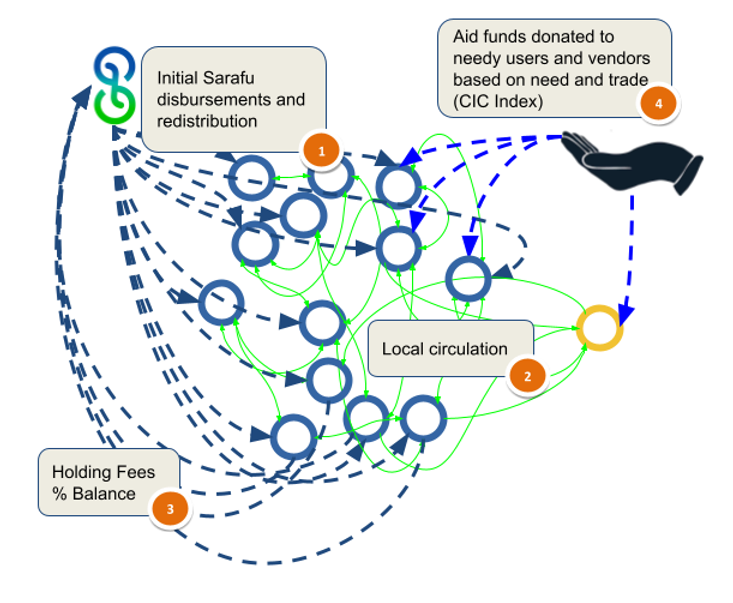
\includegraphics[width=.8\textwidth]{figures/fig_1}
    \caption{Flow of currency in the Sarafu Network. 1) Disbursements of CIC tokens are funded by donors and humanitarian organizations. Anyone is eligible to join the network and receives 400 Sarafu (\$3.60 nominal or \$9.73 PPP) upon mobile registration. 2) Sarafu circulation is kick-started within the community when key hubs such as businesses and schools agree to accept the currency. New users are incentivized to join through community workshops and word of mouth. 3) Holding fees (“negative tax” or “demurrage”) encourage users to spend their Sarafu. 4) Donor organizations can use anonymized trade data from to target user groups in need of capacity-building e.g. female farmers, healthcare workers, teachers, etc. (Image source: Grassroots Economics, 2021)}
    \label{fig:fig1}
\end{figure}


Today, the Sarafu network has over 40K users across Kenya in both rural and urban communities (see \autoref{fig:fig3}). Roughly 38\% of users are male, 31\% are female, and 31\% have unknown or “other” gender. The majority of trade goes toward food and water, communal table-banking groups (locally known as chamas), farming and labour, and retail stores. Internal research by GE in 2018 concluded that the majority of users live on less than \$1 per day. Results from a 2020 Kenya Red Cross survey suggest that the majority of Sarafu users are between the age of 26-36 and have a mean household size of 4 people. 70\% of users believe that using Sarafu has helped them access goods they otherwise would not be able to buy, and nearly 80\% believe Sarafu has helped them save more in Kenyan Shillings \citep{Kenya2020}.

\begin{figure}[hp]
    \centering
    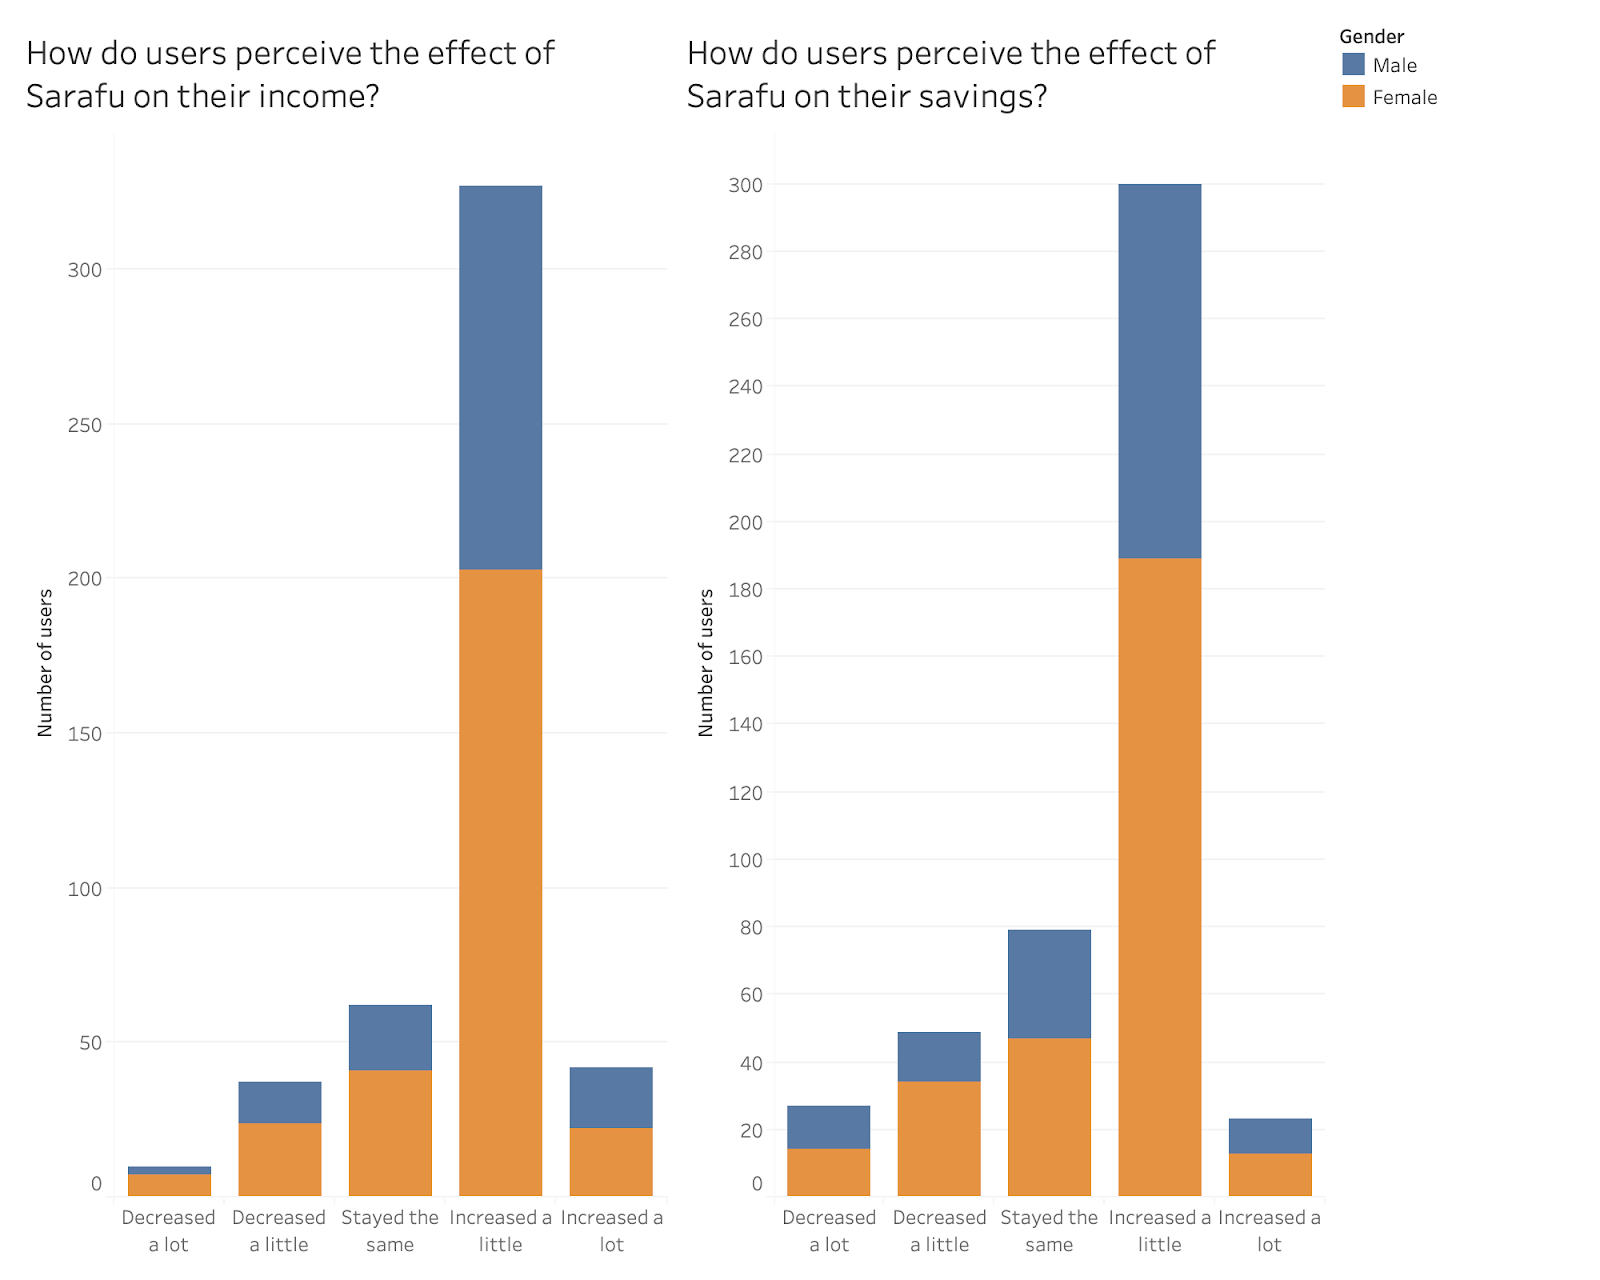
\includegraphics[width=.9\textwidth]{figures/fig_2}
    \caption{Perceptions of the effect of Sarafu on income and savings (Kenya Red Cross, 2020)}
    \label{fig:fig2}
\end{figure}

\begin{figure}[hp]
    \centering
    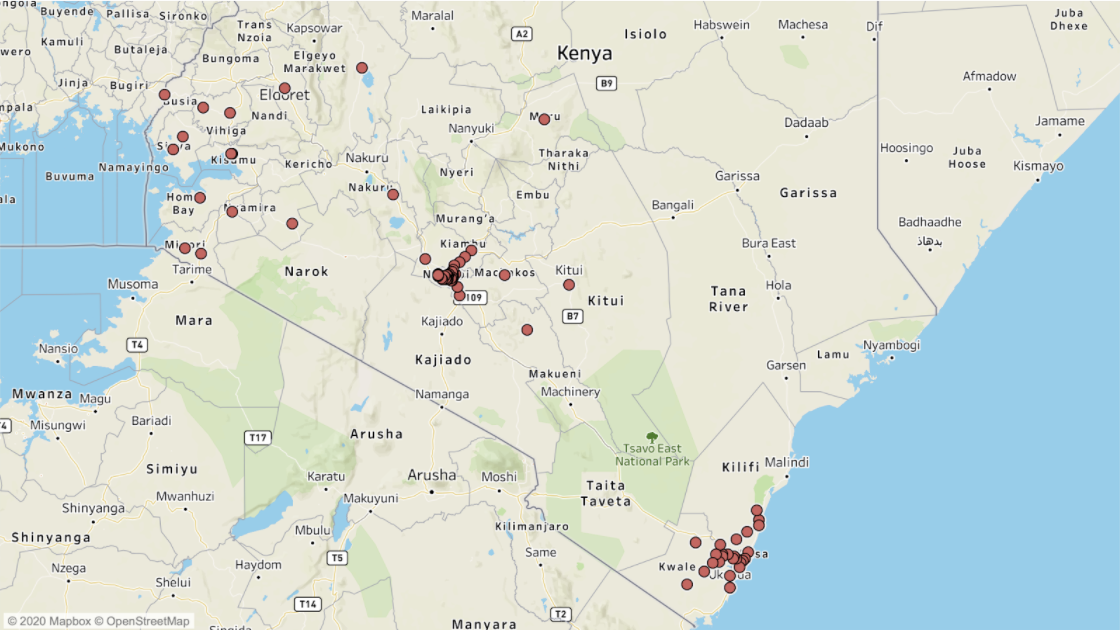
\includegraphics[width=\textwidth]{figures/fig_3}
    \caption{Geographical distribution of Sarafu users (circles represent clusters)}
    \label{fig:fig3}
\end{figure}

\begin{figure}[hp]
    \centering
    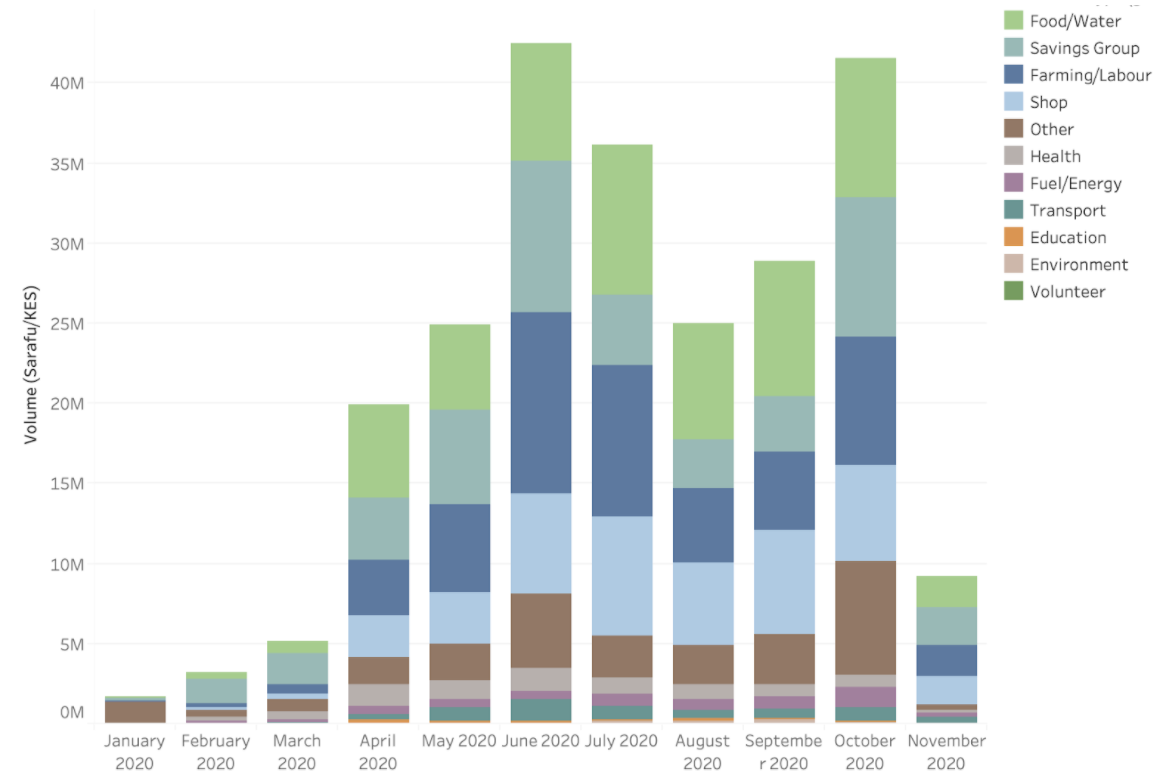
\includegraphics[width=.9\textwidth]{figures/fig_4}
    \caption{Sarafu monthly trade volume by category (Grassroots Economics, 2020)}
    \label{fig:fig4}
\end{figure}

\section{Study design}
\label{sec:section5}
This study consisted of randomization at the individual level, where treatment and control units were drawn from an eligible population of Sarafu users in Nairobi. Two research questions are explored, with their relevance in the literature and accompanying hypotheses described below:

\begin{enumerate}
    \item \textit{As a crisis recovery tool, what effect do CIC transfers have on the local economic engagement of recipients?} If this effect is negligible, then we would expect to see no significant change in trading behaviour beyond the nominal increase equal to the transfer amount. If this effect is meaningful, it would suggest CICs are an effective tool for addressing individual welfare needs and rebuilding fragile economies in the wake of aggregate shocks. Previous studies on cash transfer programs have shown higher returns to capital for beneficiaries running small businesses \citep{de2007returns}, larger asset holdings (GiveDirectly, 2013), a greater appetite to invest (Gertler et al., 2013) and overall higher consumption levels (Give Directly, 2013; \citep{egger2019general}). We would expect CIC transfers to have at-least similar effects.\\
    \textbf{Hypothesis 1:} The impact of CIC transfers is greater than the nominal increase equal to the transfer amount and is seen in recipients’ higher trade frequency and trade volumes. Furthermore, because these impacts undergo the local multiplier effect, positive economic spillovers are distributed within the immediate community and therefore support local economic recovery.

    \item \textit{Do CC transfers display the same effects for women and men?} If there are significant differences in treatment effects skewed against women, this may point to the role of economic gender imbalances. Alternatively, if treatment effects are higher for women, this may point to CICs as a tool for gender empowerment. Existing literature presents mixed results in this regard. It is widely acknowledged that simply receiving cash transfers does not necessarily empower female beneficiaries as financial decision making may not be an individual decision (Tablonski et al., 2016; \citep{hagen2017impact}). Additionally, this study puts the question within the context of a global pandemic, where women have been hit the hardest on almost every front.\\
    \textbf{Hypothesis 2:} The positive economic impacts of emergency CIC transfers are augmented for women.
\end{enumerate}

In addition to answering these research questions, the study aims to pilot a fully-remote RCT and illustrate the viability of low-cost, rapid interventions.

\subsection{Data collection}
The use of publically available, anonymized blockchain data puts a twist on the traditional RCT by eliminating the need for costly user surveys. Baseline characteristics are pulled directly from the blockchain, including gender, location, and detailed spending patterns based on every transaction ever recorded. This gives an accurate map of how users interact with the Sarafu Network and makes it easier to determine treatment and control groups. Furthermore, all outcome variables of interest are also pulled from trade data, ensuring accurate impact evaluation based on actual spending data and not self-reported results. This novel application of a remote RCT illustrates what is possible when highly detailed, anonymized data is made publicly and freely available. Cost can be a constraining factor when it comes to data collection, as baseline surveys often require field work, time and money. Although it is permissible to omit this step under certain conditions, baseline surveys are still widely used to isolate the impact of a program and check that randomization was conducted appropriately. \cite{duflo2007using} note that “the alternative strategy of collecting ‘pre-intervention data’ retrospectively in the postsurvey will usually be unacceptable, because even if the program does not affect those variables it may well affect recall of those variables.” On the other hand, the authors argue administrative data (“data collected by the implementing organization as part of their normal functioning”) could introduce biases based on prior data collection methods. The cost of producing suitable baseline data together with the cost of impact evaluation can quickly drive up a study’s budget into the thousands and hundreds of thousands. For example, \citep{speich2019resource} found that the median preparation cost for an RCT in 2016 was \$72,600. For studies on UCTs, the numbers are even more staggering: total program costs excluding transfer amounts and evaluation expenses for a 2019 joint study by Give Directly and IDInsight cost nearly \$930,000 – the equivalent of giving \$1,000 to approximately 900 additional households \citep{cook2019cash}.

\subsection{Sample selection}
\autoref{fig:fig5} provides an overview of the sample selection process and \autoref{fig:fig6} shows the geographical distribution of the final study sample in Nairobi. Eligibility criteria were applied as follows:

\begin{enumerate}
    \item The Sarafu population was filtered to include only users living in Nairobi County.
    \item Wallets belonging to savings groups or GE system administrators were removed from the data to restrict transfers to individual wallets.
    \item Wallet addresses were filtered such that only individuals who had been active for at least 30 days and traded at least once per week were eligible for participation.
    \item Individuals were randomly assigned to treatment and control, with the proportion of each group determined by calculating the sample size required for a 95\% confidence interval.
\end{enumerate}

389 individuals were assigned to treatment and 402 were assigned to control. Within the treatment group, 186 were male (47.81\%) and 203 were female (52.19\%). Within the control group, 172 were male (42.78\%) and 230 were female (57.21\%). This shows a slight deviation from the overall gender distribution in the Sarafu Network population, where (excluding unknown gender labels) 56.05\% are male and 43.95\% are female.

\begin{figure}[hp]
    \centering
    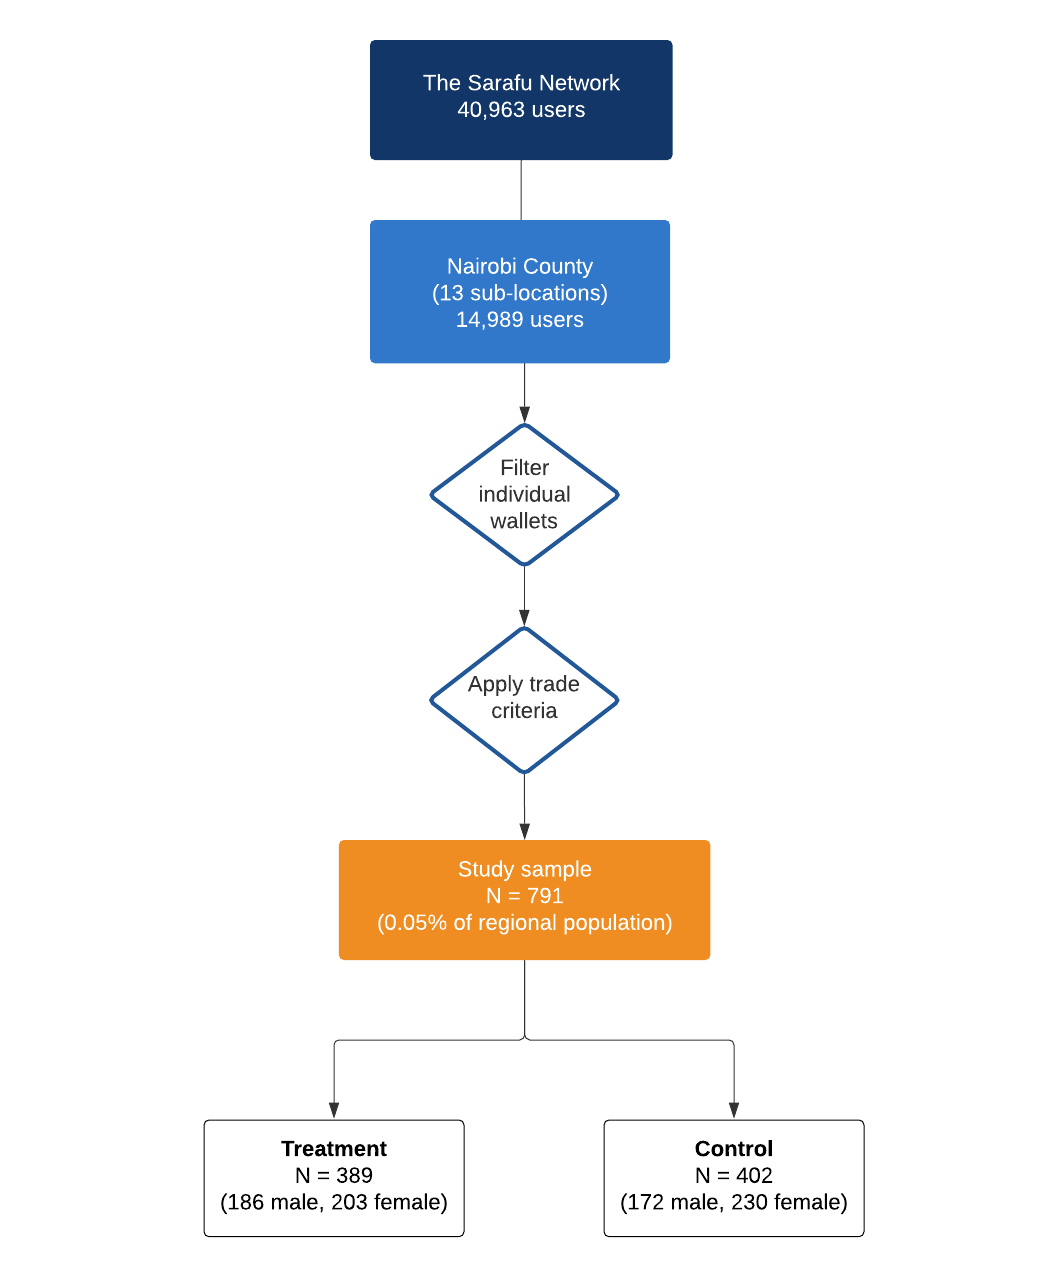
\includegraphics[width=.9\textwidth]{figures/fig_5}
    \caption{Schematic diagram of the sample selection process}
    \label{fig:fig5}
\end{figure}

\begin{figure}[H]
    \centering
    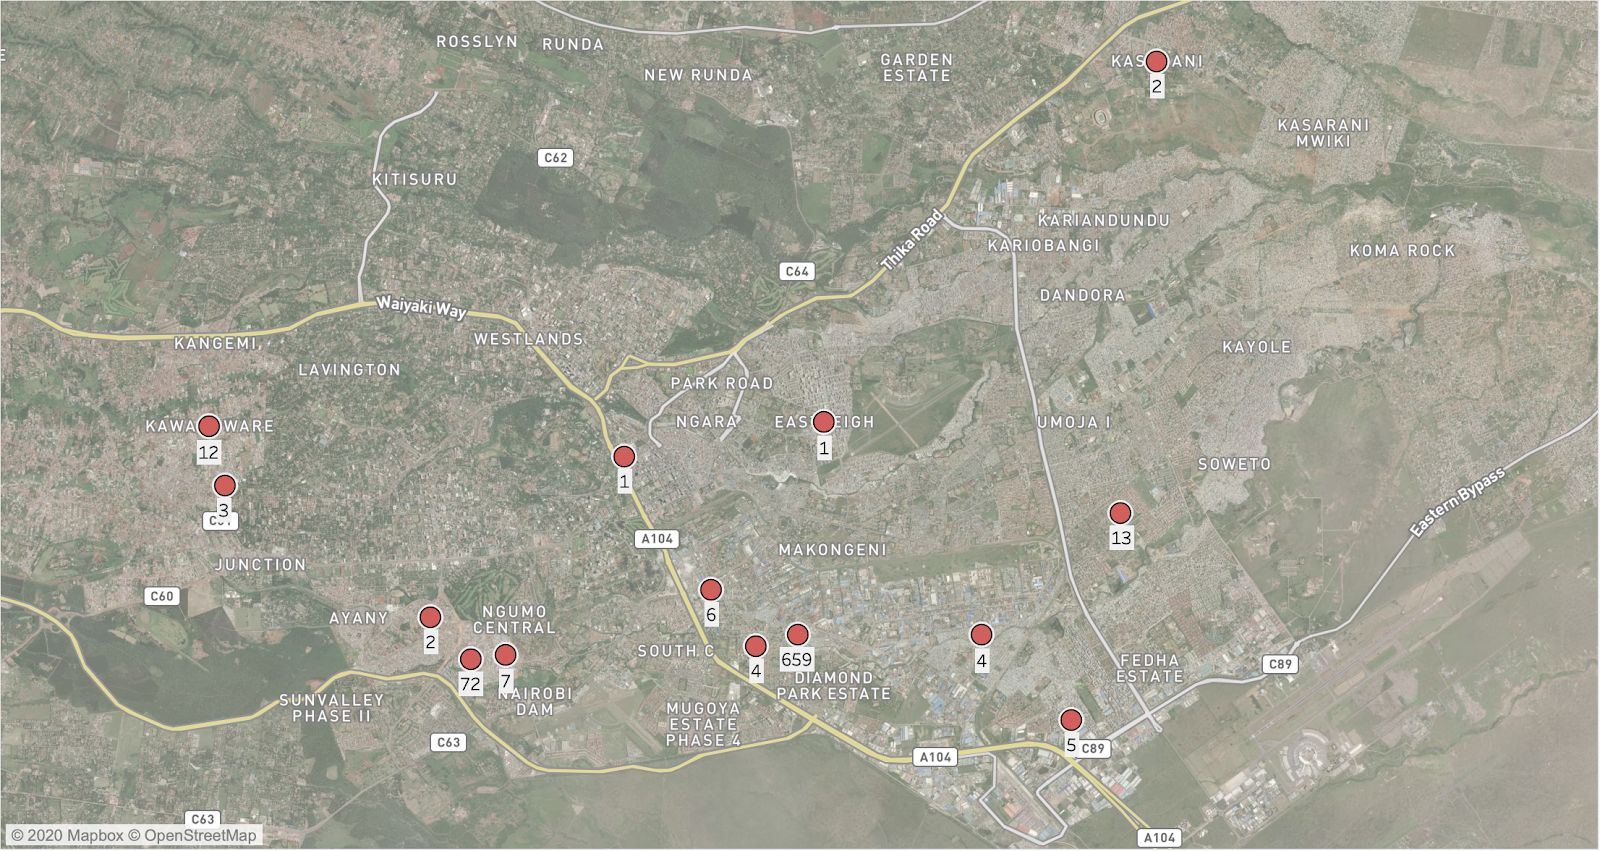
\includegraphics[width=\textwidth]{figures/fig_6}
    \caption{Location clusters of sample units in Nairobi}
    \label{fig:fig6}
\end{figure}

\subsection{Intervention}
Individuals in the treatment group received a flat transfer of 400 Sarafu CIC tokens each week for three consecutive weeks, beginning on 20 November 2020 and ending on 4 December 2020. Each round was accompanied by an SMS informing the recipient of the transfer and providing a shortcode to check their new account balance.

\begin{figure}[H]
    \centering
    
\includegraphics[width=\textwidth]{figures/fig_7}
    \caption{English/Swahili text messages sent to transfer recipients}
    \label{fig:fig7}
\end{figure}

The transfer amount corresponds to the credit bonus new users receive when registering on the network for the first time as well as just lower than the average user balance in Nairobi. Since Kenya has a purchasing power parity of 41.1, this means for every \$1 received, locals can buy 2.43 times the amount of goods in community currency than they would buy in the United States using US dollars. A transfer of 400 Sarafu worth \$3.60 (nominal) therefore corresponds to a purchasing power of \$9.73. The total value of all transfers is 1,200 Sarafu or \$29.20 PPP. \autoref{tab:tab1} provides a rough idea of what this amount of money can buy.

\begin{table}[h]
    \centering
    \caption{Cost of basic goods in Kenyan Shillings and USD PPP adjusted prices}
    \label{tab:tab1}
    \begin{tabular}{p{3.5in}cc} \hline
     & (1) & (2) \\
    Item & Approx. local price & USD PPP \\
	 & in KES & adjusted price \\ \hline
    2kg maize meal & 105 & 2.55 \\
    1L refined vegetable oil & 352 & 8.56 \\
    500g bread & 43 & 1.05 \\
    500ml cow's milk & 45 & 1.09 \\
    1L gasoline & 106.3 & 2.59 \\
    1L diesel & 91.8 & 2.23 \\
    One-way boda-boda ride ($<$10 km) & 80 & 1.95 \\ \hline
    \multicolumn{2}{l}{\textit{Source: Famine Early Warning Systems Network (2020)}} \\
    \end{tabular}
\end{table}

Although small-scale weekly transfers were selected in favour of a large lump sum payment due to budget constraints, research suggests that the effects of smaller transfers on food consumption, asset accumulation and economic participation are comparable to graduation type programs commonly evaluated in the literature, and may even have larger multiplier effects on productivity and income \citep{handa2018can}.

\subsection{Baseline statistics}
The list of baseline variables used in the econometric specification in \autoref{eq:eq3} are described below in \autoref{tab:tab2}. Baseline balance tests have been purposefully omitted from this analysis as there is a weight of research that suggests these methods are only informative when there is reason to believe randomization was not carried out correctly or when attrition is high. In all other cases, baseline balancing undermines the concept of randomization by attempting to assign a probability to an event that by design should occur through chance (Altman, 1985; \citep{bruhn2008pursuit}). Differences between baseline characteristics in treatment and control groups were instead analyzed using a standardized mean difference (SMD) score, reported in \autoref{tab:tab3}. SMD provides a measure of the distance between two group means, enabling a meaningful comparison across variables of different scales. This is similar to the approach proposed by Imbens and Rubin (2015), who argue that the focus of baseline balancing should not be on statistical significance but rather on the size of differences. An SMD greater than 0.1 is often considered a sign of important covariate imbalance. Only 2 out of 11 covariates showed values greater than 0.1. Other baseline characteristics for trade activity are fairly comparable across treatment and control, hence in the economic specification detailed in \autoref{eq:eq3}, the expected correlation between the error term $\varepsilon_i$ and treatment status is zero.

\begin{table}[h]
    \centering
    \caption{Baseline controls (recorded one day before treatment intervention)}
    \label{tab:tab2}
    \begin{tabular}{p{2in}p{4in}} \hline
    Wallet Balance (USD) & The USD value of CIC tokens held in a user's wallet \\
    Total Income (USD) & The total volume that has entered a user's wallet through sales since enrolment \\
    Total Expenditure (USD) & The total volume that has left a user's wallet through purchases since enrolment \\
    N. Sales & The total number of trades in which a user received money \\
    N. Purchases & The total number of trades in which a user spent money \\
    Trade Network Size (In) & The total number of unique trade partners who have sent a user money \\
    Trade Network Size (Out) & The total number of unique trade partners who a user has sent money to \\
    Food/Water (USD) & The total volume spent by a user on food or water \\
    Education (USD) & The total volume spent by a user on educational expenses \\
    Health (USD) & The total volume spent by a user on health expenses \\
    Savings (USD) & The total volume spent by a user on savings (typically through table banking groups locally known as \textit{chamas}) \\ \hline
    \end{tabular}
\end{table}

\begin{table}[h]
    \centering
    \caption{Baseline statistics with standardized mean differences (SMD)}
    \label{tab:tab3}
    \begin{tabular}{lccc} \hline
    & Control Mean & Treatment Mean & SMD \\
    & (Std. Dev.) & (Std. Dev.) & \\ \hline 
    Wallet Balance (USD) & 2,793.36 & 2,823.54 & 0.005 \\
    & (7048.84) & (5405.33) & \\
    Total Income (USD) & 2709.12 & 2733.98 & 0.004 \\
    & (7025.49) & (5374.22) & \\
    Total Expenditure (USD) & 2739.95 & 2754.99 & 0.002 \\
    & (7004.60) & (5373.38) & \\
    N. Sales & 119.06 & 137.54 & 0.115 \\
    & (122.71) & (190.50) & \\
    N. Purchases & 121.38 & 127.41 & 0.043 \\
    & (116.55) & (159.92) & \\
    Trade Network Size (In) & 32.74 & 30.62 & 0.101 \\
    & (26.23) & (21.98) & \\
    Trade Network Size (Out) & 30.38 & 27.16 & 0.011 \\
    & (19.96) & (19.29) & \\
    Food/Water (USD) & 755.12 & 779.46 & 0.019 \\
    & (1427.97) & (1122.95) & \\
    Education (USD) & 12.53 & 11.82 & 0.01 \\
    & (87.25) & (49.00) & \\
    Health (USD) & 62.97 & 87.56 & 0.089 \\
    & (211.04) & (326.41) & \\
    Savings (USD) & 308.08 & 285.98 & 0.033 \\
    & (699.24) & (644.03) & \\ \hline
    \textit{N} & \textit{402} & \textit{389} & \\ \hline
    \end{tabular}
\end{table}

\subsection{Study integrity}
\subsubsection{Compliance}
CIC transfers were sent via the xDAI blockchain to specified wallet addresses, therefore all treatment units were in fact treated.

\subsubsection{Attrition}
If attrition is correlated with treatment assignment, this could potentially bias estimates for program impact. Attrition is unlikely to have meaningfully biased the results of this experiment as subjects were selected from an existing group of active Sarafu users and the treatment intervention – a free disbursement of tokens – made opt-out unlikely.

\subsubsection{Spillover effects}
Rubin’s causal model asserts that for accurate causal inference, the stable unit treatment value assumption (SUTVA) must hold – in other words, that the potential outcomes observed for one unit should not be affected by the treatment assignment of other units \citep{rubin1990formal}. This includes effects that operate economically, such as through an increase in local trade and psychologically, such as through John Henry effects, where members of the control group behave differently because they are aware they are being compared to the experimental group. However, \cite{thome2016local} note that by design, cash transfers generate spillovers when households other than those assigned to treatment are affected by the inflow of money to the local economy. This is due to changes in “incomes, production, consumption decisions, access to information, perceptions or even social interactions”. Some flexibility must be allowed for within-region spillovers, where treated and control units are almost guaranteed to interact with each other. For example, when a transfer beneficiary buys their food from an individual in the control group, the beneficiary’s increase in expenditure corresponds with the non-beneficiary’s increase in income.

There are two general approaches in the literature to address this kind of interference. First, some programs will include a “pure control” in a different region where units are guaranteed to not have interacted with the treatment group. In this study, however, such a design feature was not possible due to the small sample size in other eligible regions. The second approach is to use some objective function to capture the distribution of these spillovers within the community. This study does not attempt to model these effects precisely and acknowledges that even existing methods such as Social Accounting Matrix (SAM) linear multipliers and Keynesian transfer multipliers are often applied with limited data in an approximate manner (see \cite{egger2019general}; Taylor, 2013; Thome, 2013 and 2016; Sadoulet et al., 2001, etc.) In the context of CICs, economy-wide multipliers are not suitable without additional data on the circulation of national currency, local labour supply and other baseline characteristics. However, it may still be useful to isolate a simple expenditure multiplier for the CIC economy based on the principles of Taylor’s “local economy-wide impact evaluation” (LEWIE) multiplier, which has been used in a number of cash transfer programs. The LEWIE model first applies Monte Carlo methods on parameter estimates to generate simulated results. The multiplier is then calculated by taking the sum of recipients’ and non-recipients’ total value change in an outcome of interest and dividing it by the total amount transferred. The multiplier therefore indicates the additional monetary value generated for an outcome of interest for each US dollar transferred. The multiplier’s difference in magnitude between groups also indicates the treatment effect on the size of positive spillovers. A multiplier that is greater than zero for non-beneficiaries and greater than one for beneficiaries is evidence of positive feedback effects between the two groups. For example, if a treated individual’s increase in expenditure is greater than the total transfer amount, then the additional spending volume can be attributed to these positive spillover effects. In Section 5 (Results), the mean expenditure multiplier reported for each cohort is calculated as follows:

\begin{equation}
    M_{X_{t}}=\frac{1}{N} \sum_{i=0} \frac{X_{i, t}-X_{i, t-1}}{K}
    \label{eq:eq1}
\end{equation}

Here $M_{X_{t}}$ is the mean expenditure multiplier measured post-treatment for the group, $N$ is the group's sample size, $X_{i, t}$ is an individual's non-durable expenditure post-treatment, $X_{i, t-1}$ is the value of their non-durable expenditure measured at baseline, and $K$ is the transfer amount.

\subsection{Analysis period and outcome variables}
Treatment and control wallets were tracked from the beginning of the study period to two months after the final transfer. \autoref{tab:tab4} provides a detailed description of each outcome variable.

\begin{table}[h]
    \centering
    \caption{Individual outcome variables measured post-treatment (USD PPP adjusted where relevant)}
    \label{tab:tab4}
    \begin{tabular}{p{2.1in}p{4in}} \hline
    Variable & Description \\ \hline
    Wallet Balance (USD) & The USD value of CIC tokens held in a user's wallet \\
    Monthly Income (USD) & The total volume that entered a user's wallet through sales in the past month \\
    Monthly Expenditure (USD) & The total volume that left a user's wallet through purchases in the past month \\
    Marginal Propensity to\newline Consume & The proportion of a user's increase in income that was spent rather than saved during the past month \\
    Ave. Trade Size (USD) & A user's average purchase amount during the past month \\
    Food/Water (USD) & A user's total expenditure on food or water in the past month \\
    Savings (USD) & A user's total expenditure on savings in the past month (typically through table banking groups locally known as chamas) \\ \hline
    \multicolumn{2}{p{6.2in}}{Notes. For each measurement period analyzed (i.e. one week after the final transfer and two months after the final transfer), outcome variables are measured relative to the past month. The first measurement period therefore looks at the month during which transfers were distributed.}
    \end{tabular}
\end{table}

Marginal propensity to consume (MPC) measures the increase in consumer spending that can be attributed to a change in disposable income. The standard Keynesian formula is used, captured in \autoref{eq:eq2} below:

\begin{equation}
    M P C=\frac{\Delta C}{\Delta I}
    \label{eq:eq2}
\end{equation}

Here $\Delta C$ is change in spending, calculated as a user’s total volume traded out measured post-treatment minus their total volume traded out at baseline. $\Delta I$ is change in disposable income, calculated as a user’s total income measured post-treatment minus their total income measured at baseline.

\subsection{Econometric specifications}
The treatment effect of CIC transfers is captured in \autoref{eq:eq3} below:

\begin{equation}
    y_{i}=\beta_{0}+\beta_{1} T_{i}+\beta_{2} F_{i}+\beta_{3}\left(T_{i} \times F_{i}\right)+\delta_{i B}+\varepsilon_{i}
    \label{eq:eq3}
\end{equation}

Here $y_{i}$ is the outcome of interest for individual $i$ (with each outcome described in Table4), $\beta_{0}$ is the constant term, $T_{i}$ is a binary treatment indicator that takes the value 1 for individuals in the treatment group (i.e. Sarafu users who received CIC transfers) and 0 for individuals in the control group (i.e. Sarafu users who did not receive CIC transfers), $F_{i}$ is binary sex indicator that takes the value 1 for females and 0 for males; $\delta_{i B}$ is the set of baseline adjustments described in \autoref{tab:tab2}, $\left(T_{i} \times F_{i}\right)$ is an interaction term to compare the relative effects on treated females and $\varepsilon_{i}$ is an error term. Following McKenzie (2012), baseline terms are included alongside standard demographic controls. This improves statistical significance by accounting for random imbalances in variables that were not controlled during the study selection process. In addition, the baseline values used in \autoref{eq:eq3} are not the same as those used for determining original study eligibility; instead, baseline values for outcome variables were re-measured exactly one day before the first transfer in order to improve the accuracy of interpretations on the treatment effect. Because of the large number of outcome variables in this study, the likelihood of Type 1 errors (falsely rejecting the null hypothesis), also known as the family-wise error rate (FWER), increases with each additional variable (Clark, 2019; McKenzie, 2020). In order to address these issues of multiple inference, Romano-Wolf stepdown adjusted p-values are applied.


\section{Results}
\label{sec:section6}
\subsection{Overall impacts}
\autoref{tab:tab5} shows the basic treatment effect on the outcome variables detailed in \autoref{tab:tab4} two months after the final transfer round. Column (1) reports the coefficient $\beta_1$ on the treatment indicator as described in \autoref{eq:eq3}. In parentheses are the upper and lower bounds for the 95\% confidence interval of this treatment effect. Note that the reported significance levels are those taken before applying the Romano-Wolf FWER correction for multiple inference, after which none of the significance levels survived.

\begin{table}[h!]
    \centering
    \caption{Treatment effects on outcome variables after two months}
    \label{tab:tab5}
    \begin{tabular}{lcc} \hline
     & (1) & (2) \\
    Outcome & Treatment effect & Female recipient \\
	 & (95\% CI) & (95\% CI) \\
	 & [Adjusted p-value] & [Adjusted p-value] \\ \hline
	 Wallet Balance (USD) & 93.51 ** & -85.18 \\
	 & (12.75, 174.26) & (-214.70, 44.34) \\
	 & [0.22] & [0.52] \\
    Monthly Income (USD) & 23.17 ** & -40.67 ** \\
     & (0.03, 46.31) & (-79.00, -2.33) \\
     & [0.26] & [0.20] \\
    Monthly Expenditure (USD) & 16.30 * & -26.88 \\
     & (-0.76, 33.37) & (-62.87, 9.11) \\
     & [0.26] & [0.48] \\
    Marginal Propensity to Consume & 0.60 ** & -0.89 ** \\
     & (0.03, 1.17) & (-1.65, -0.13) \\
     & [0.26] & [0.17] \\
    Ave. Trade Size (USD) & 6.31 * & -3.89 \\
     & (-0.26, 12.87) & (-15.09, 7.32) \\
     & [0.26] & [0.55] \\
    N. Sales & 2.97 ** & -3.34 * \\
     & (0.53, 5.40) & (-7.16, 0.47) \\
     & [0.21] & [0.36] \\
    N. Purchases & 2.47 ** & -2.00 \\
     & (0.21, 4.72) & (-5.69, 1.70) \\
     & [0.26] & [0.54] \\
    Food/Water (USD) & 28.43 * & -29.39 \\
     & (-0.54, 57.40) & (-73.56, 14.79)\\
     & [0.25] & [0.52] \\ \hline
    \multicolumn{3}{p{6in}}{\textit{Notes.} OLS estimates of treatment effects two months after the final transfer. Outcome variables are listed on the left and described in detail in \autoref{tab:tab4}. Higher values correspond to positive outcomes. Column (1) reports the basic treatment effect comparing indivduals in the treatment group to individuals in the control group. Column (2) reports the relative treatment effect of transfering CIC tokens to females compared to males. For each outcome variable listed in columns (1) and (2), the coefficient on the treatment or treated female indicator is reported with the 95\% confidence interval in parentheses. Standard model p-values are indicated with asterisks alongside coeffcients while Romano-Wolf FWER corrected p-values are shown in square brackets.} \\
    \\
    \multicolumn{3}{p{5.5in}}{Significance codes: * p$<$0.1, ** p$<$0.05, *** p$<$0.01} \\
    \end{tabular}
\end{table}

After two months, statistically significant and economically meaningful impacts of CIC transfers were found for beneficiaries’ wallet balance, monthly income, monthly expenditure, marginal propensity to consume, average trade size, number of sales, number of purchases and expenditure on food and water. Beneficiaries’ wallet balance was larger than the control group by \$93.51 and their marginal propensity to consume was 0.60 points higher, with both results statistically significant at the 5\% level. Beneficiaries had a monthly CIC income \$23.17 higher than the control group (significant at the 5\% level) and spent \$16.30 more (significant at the 10\% level). During the study period, beneficiaries traded more frequently and in larger amounts, showing an average trade size \$6.31 higher than individuals in the control group (significant at the 10\% level), with 2.97 more sales and 2.47 more purchases (both significance at the 5\% level). There was also a \$28.43 increase in beneficiaries’ expenditure on food and water within the CIC network, statistically significant at the 10\% level.

After applying the transfer multiplier discussed in Section 5.5.3, beneficiaries had a mean expenditure multiplier of 8.28 while non-recipients had a mean expenditure multiplier of 6.69. Since the increase in expenditure for both groups is considerably greater than the nominal transfer amount, this is an indication of positive spillover effects.

Overall, these findings support the hypothesis that CIC transfers boost the local economic engagement of recipients, thus catalyzing individual and community-level recovery in the wake of aggregate shocks. The difference in food expenditure supports previous research that highlights CICs as an effective policy tool for fighting food insecurity (Cauvet 2014; Santos, 2017; Zeller, 2020). The results are also consistent with more recent studies on the impact of cash transfers in response to the Covid-19 pandemic – for example, \cite{banerjee2020effects} found that recipients in Kenya were 4.9 to 10.8 percentage points less likely to experience hunger relative to the control group mean of 68\%. While the results of this study do not tell us how food expenditure has affected hunger levels or nutrition, the size of the treatment effect is over two thirds the transfer amount, suggesting that recipients placed a higher level of importance on securing more food than they did on expenses such as education, healthcare or savings. These impacts suggest that CIC transfers are primarily used for consumption, echoing similar findings in the literature where short-term cash transfers tend to be correlated with increased consumption (Haushofer \& Shapiro, 2016).

\subsection{Gender differences}
The coefficients in Column (2) for the relative treatment effect on female recipients suggest that gender imbalances play a strong role in determining the impact of emergency CIC transfers. This disproves the hypothesis that positive transfer impacts are amplified for female beneficiaries. Before exploring this variation in results, several constraints must be acknowledged:

\begin{enumerate}
    \item The majority of the coefficients in Column (2) lack statistical significance and therefore limit any conclusive generalizations.
    \item A natural limitation of this data is that it only tells us about treatment effects on the CIC economy. For every CIC-based outcome, there is a parallel outcome denominated in national currency whose relationship with the former remains unknown. Currently there exists little to no theory in this area; while this paper does not attempt to explain this relationship, it highlights a crucial point for further research.
\end{enumerate}

After two months, female beneficiaries experience a positive treatment effect on their wallet balance (\$85.18 or 91\% lower than the treatment effect on males), a negative treatment effect on monthly CIC income, a negative treatment effect on monthly CIC expenditure, a negative treatment effect on marginal propensity to consume, a positive treatment effect on average trade size (\$3.89 or 62\% lower than the treatment effect on males), a positive treatment effect on number of sales (2 units lower than treated males), a negative treatment effect on number of purchases, and a negative treatment effect on food and water expenditure.

Based on their higher marginal propensity to consume, average trade volume and number of sales and purchases, it is reasonable to conclude that male beneficiaries on the whole were less conservative with how they spent their transfers, potentially amplifying positive spillover effects well after the intervention was completed. This is consistent with literature that suggests cash transfers encourage risk taking and thus an expansion of business opportunities for individuals and small enterprises \citep{banerjee2020effects}.

On the other hand, while females also showed small positive treatments effects on their wallet balance and average trade size, the negative treatment effect on monthly CIC income, monthly CIC expenditure, marginal propensity to consume, and food and water expenditure is a strong indicator that female beneficiaries were more cautious than even the control group in how they chose to spend their additional income during the study period. In light of this, it may be more useful to interpret the coefficient on marginal propensity to consume as a behavioural indicator which helps partially explain the variation observed in other outcomes. Finally, it bears emphasizing that the effects on CIC income and expenditure may indicate female beneficiaries’ preference to trade outside of the CIC network for any number of unknown reasons. One plausible explanation is that female beneficiaries may have exhausted their transfers on immediate consumption needs (i.e. through trade with other members of the Sarafu network) and thereafter chosen to trade exclusively outside of the CIC network in search of more trade partners.

\autoref{fig:fig8} and \autoref{fig:fig9} show multiple graphs with the predicted values and mean treatment effects after running 1,000 Monte Carlo simulations on the regression coefficients in \autoref{tab:tab5}. On the left, the boxplots show the distribution of simulated values for each outcome variable by cohort. On the right, the treatment effect for the outcome variable is analyzed by gender. The discussion that follows analyzes these differences on multiple levels of analysis: first, in the context of existing gender disparities in Sarafu Network and the broader Kenyan economy, and secondly, in the context of the Covid-19 pandemic and its disproportionate impacts on women.

\begin{figure}[H]
    \centering
    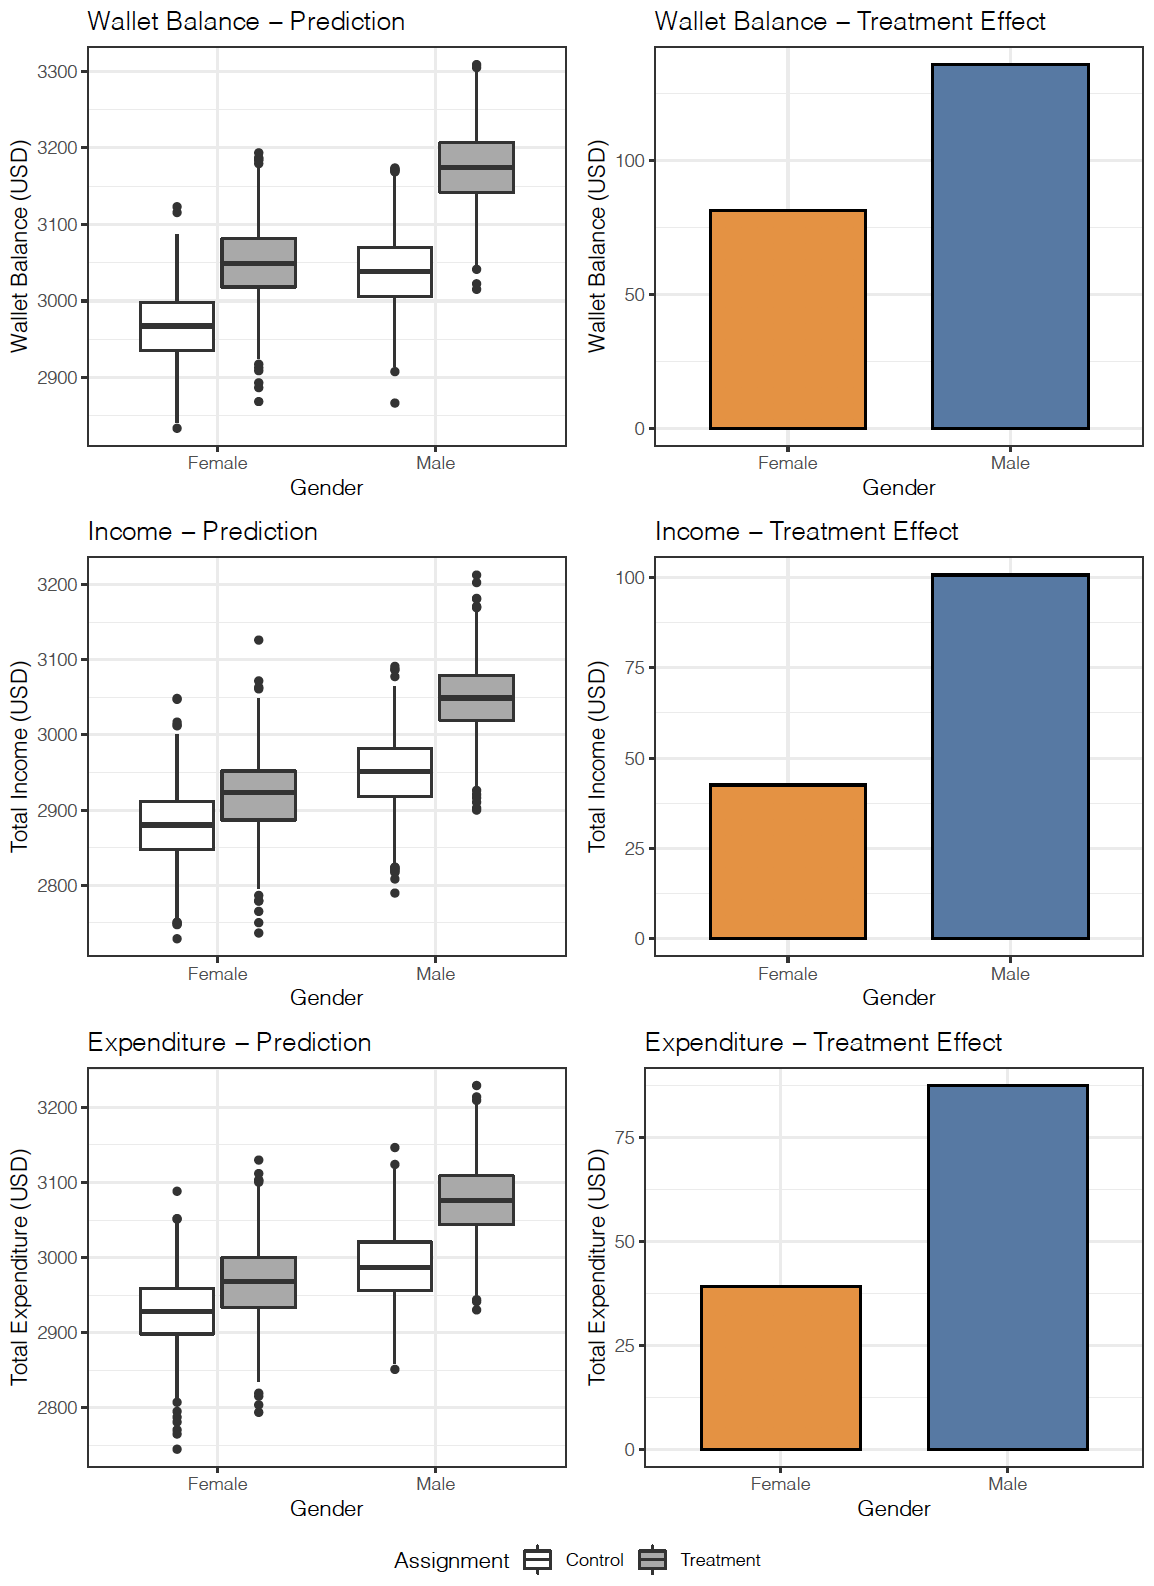
\includegraphics[width=0.95\textwidth]{figures/fig_8}
    \caption{Outcome predictions by cohort (left) and treatment effects by gender (right)}
    \label{fig:fig8}
\end{figure}

\begin{figure}[H]
    \centering
    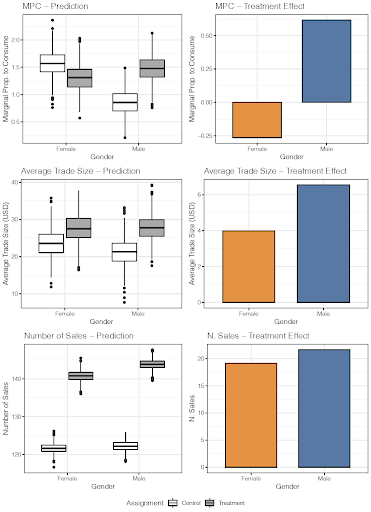
\includegraphics[width=0.95\textwidth]{figures/fig_9}
    \caption{Outcome predictions by cohort (left) and treatment effects by gender (right)}
    \label{fig:fig9}
\end{figure}

The variations observed in both regression and simulated results echo gender imbalances throughout Kenya’s economy and within the Sarafu network itself. Women tend to be less mobile and have lower market participation due to cultural norms and other constraints \citep{bergman2019gendered}. In the Sarafu network, more men tend to be shop owners than women – implying greater access to capital and more trade partners, which may explain why male beneficiaries could afford to be less conservative with their transfers. Motorcycle (“boda-boda”) drivers also tend to be dominated by men, increasing their mobility and access to trade opportunities (see \autoref{fig:fig10}).

\begin{figure}[H]
    \centering
    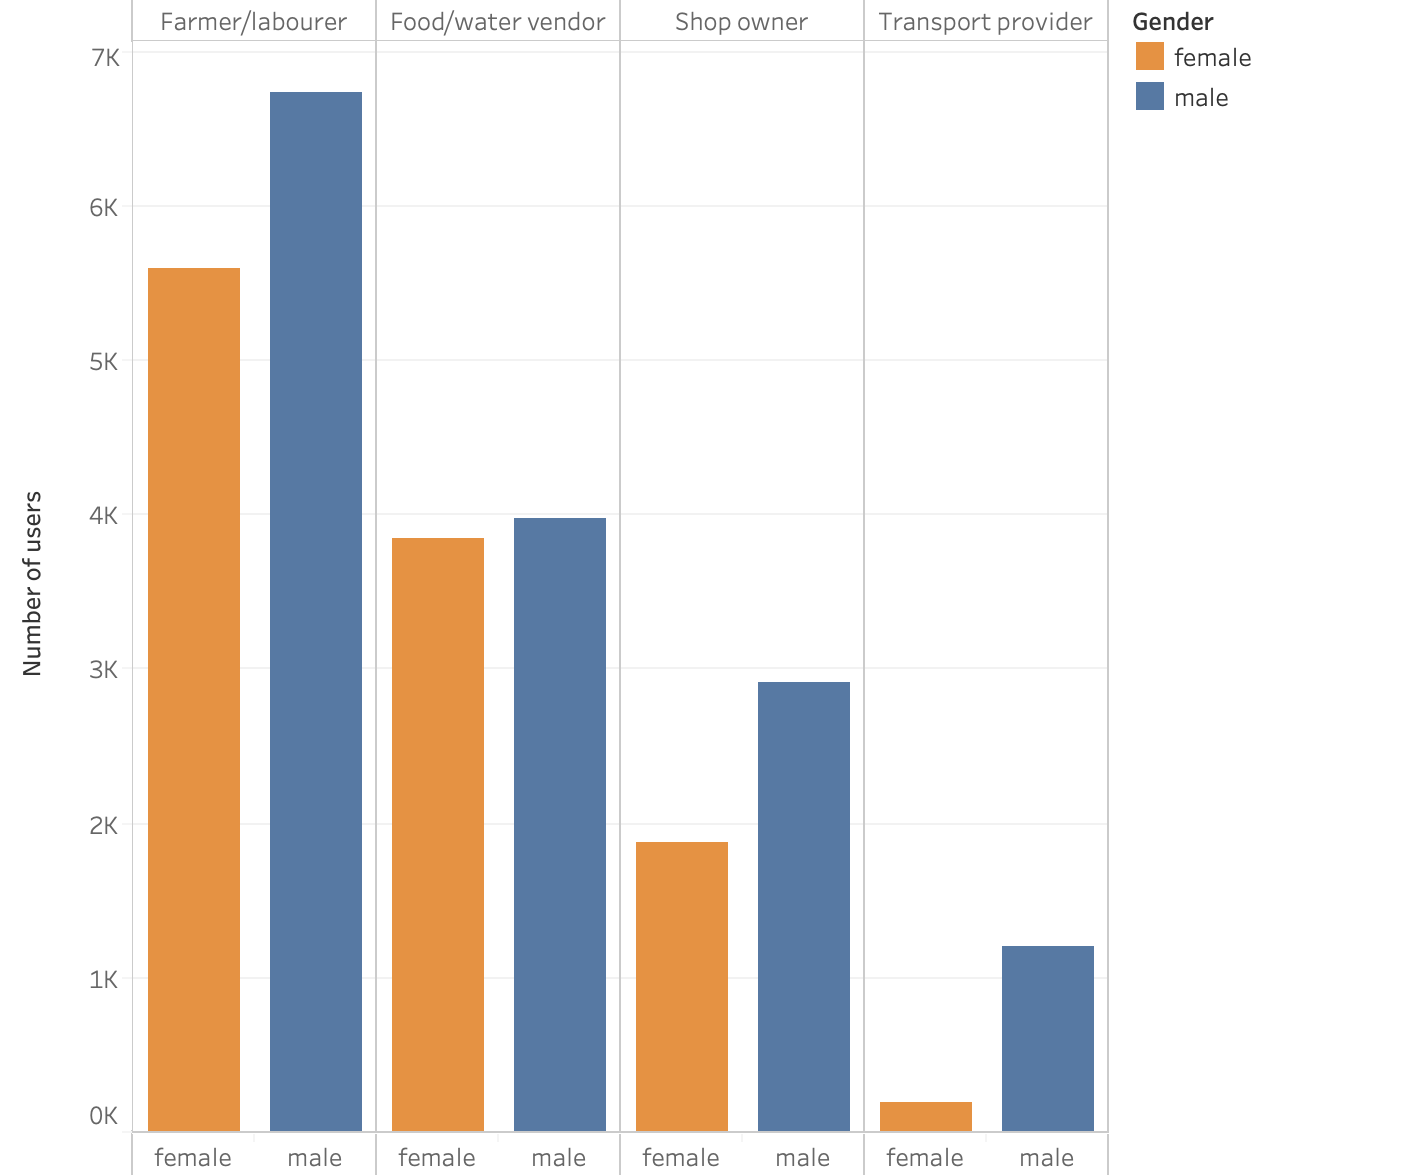
\includegraphics[width=0.95\textwidth]{figures/fig_10}
    \caption{User roles by gender (Grassroots Economics, 2021)}
    \label{fig:fig10}
\end{figure}

Finally, this study must be placed in the context of the Covid-19 pandemic, where women globally have been hit the hardest on almost every measure. Not only has this amplified existing gender disparities, but it has also influenced the financial decision making of women who must adapt to more challenging economic conditions. Ongoing data by the World Bank analyzing the effects of the pandemic on Kenyan households suggests that women have fared worse when it comes to food security and employment (World Bank, 2021). A Nairobi-based study released in late 2020 also found a stark contrast in the economic impacts of Covid-19 between young men and women \citep{Decker2021covid}. Females reported significantly more time spent on caregiving and household work and over 54\% of them reported an increase in financial reliance on others compared to 36\% of men. The researchers also note that with more men facing unemployment and being confined to the household, a skewed division of household labour has constrained women’s income generating opportunities. While these results cannot be directly translated to this study sample, they illustrate the broader context in which the impacts of Covid-19 have impeded women’s ability to work and earn. Female beneficiaries’ lower marginal propensity to consume – in other words, their more conservative spending behaviour – suggests that these women may have opted to hold on to additional income as a necessary buffer against unpredictable future cash flows.

The results from this study echo similar findings by researchers at the World Food Organization, whose eight-country case study reveals that cash transfers and vouchers have limited effects on gender empowerment when a community has experienced a large-scale disaster, but that these effects are more noticeable when communities face a smaller-scale emergency \citep{berg2013examining}. For practitioners and policymakers, this highlights the need to accompany emergency interventions with additional support targeted at females, such as temporary employment opportunities, access to microcredit and psychological services.


\section{Discussion}
\label{sec:section7}
These findings complement a growing body of work on emergency cash transfers to the poor. Overall results support the hypothesis that CICs can catalyze greater local economic engagement within a short span of time. Coupled with the quick, low-cost turnaround of the actual study implementation, this serves as an important prototype for researchers and policymakers interested in economic-based disaster-response.

However, the unique set-up of this study poses several constraints for how it is interpreted within the broader literature. Not only did recipients receive an entirely different form of currency, but they also faced extreme aggregate shocks whose impact on day-to-day living would be difficult to replicate. It is therefore necessary to decouple general cash transfers from emergency cash transfers as well as the analysis of gender empowerment from one centered on gains to one centered on economic protection. This study has also highlighted a major caveat of doing impact evaluation on closed complementary currency networks: while the data itself is accurate, we lack contextual information on users’ spending habits outside of the CIC network. As highlighted in Section 6.2, understanding the relationship between CIC expenditure and national currency expenditure continues to be a crucial missing link in the literature and should be prioritized in future research.

The consistently stronger treatment effects for males versus females raises important questions that warrant further research. In a comprehensive overview of several programs, \citep{browne2014evidence} notes a general ambiguity in the literature regarding the impact of emergency cash transfers on women, largely due to poor study designs and inadequate gender monitoring. For example, programs that only send transfers to women cannot offer direct comparability with males, limiting the discussion on empowerment to outcomes such as financial decision making or intimate partner violence. While this analysis focuses largely on differences in CIC trading behaviour, the context of the study makes any conclusive or generalized interpretation of the results somewhat misleading. For example, the question of whether to attribute these strong gender differences to the design of CIC networks versus the impact of the pandemic is impossible to answer without additional data that could be sourced from follow-up interviews.

Another area for further probing is the study design itself. While the size of these transfers was kept small due to budget constraints, an interesting follow-up would be to test the impact of larger lump-sum CIC transfers, both during periods of relative economic calm and during aggregate shocks. Previous studies suggest that larger transfers are more likely to increase investments while small transfers have a greater impact on consumption (Haushofer \& Shapiro, 2016). This study also only measured the short-term impact of CIC transfers as a crisis response tool. There is yet to be a long-term experimental study on the impact of CICs.

Finally, it is worth noting that a natural limitation of CIC networks is that because tokens can only be spent with other members of the network, recipients’ expenditure is constrained by the range of available goods and services offered by other network members within their vicinity. For example, one would not expect to see recipients open a bank account with their transfer funds because the nature of the transfer does not yet support this kind of exchangeability. Given the rapid growth of the Sarafu Network since 2018, it seems likely that with well-developed CIC networks embedded into the economy of low-income communities, future CIC transfers may show greater impacts beyond immediate spending behaviour.


\section{Conclusion}
\label{sec:section8}
The Covid-19 pandemic has exposed the fragility that underlies most local economies. It is during times such as these that we are made aware of the urgency for more effective forms of humanitarian response. Results from what is likely the first randomized control trial on community currencies suggest that even a small-scale transfer of CIC tokens can have an economically and statistically significant impact on beneficiaries, who show a \$93.51 increase in available wallet balance, a \$23.17 increase in monthly CIC income, a \$16.30 increase in monthly CIC spending, a \$6.31 increase in average trade size and a \$28.43 increase in expenditure on food and water. However, the sharp difference in treatment effects between males and females indicates that economic gender imbalances are a strong determinant of how transfers get spent. The difficulty of interpreting these differences highlights the need for further research on the relationship between CIC trade behaviour and the use of national currency, especially during socio-economic crises that disproportionately affect women. Small-scale CIC transfers used as an emergency humanitarian response should therefore be seen as an important buffer rather than as a tool for gender empowerment – although large-scale transfers are likely to yield different results.

CICs are a powerful tool for communities to change the structure of their local economy from the inside out. This model also has the potential to change how aid is administered, shifting the focus from retroactive responses to long-term liquidity retention and capacity-building. This study therefore serves as an important prototype and strengthens the case for broadening access to these models where they are needed most.


\singlespacing
\setlength\bibsep{0pt}
\bibliographystyle{apalike}
\bibliography{references}



\clearpage

\onehalfspacing


\section*{Appendix A. Resources} \label{sec:appendixa}
%\addcontentsline{toc}{section}{Appendix A}

\begin{itemize}
    \item Grassroots Economics website: \url{www.grassrootseconomics.org}
    \item \href{https://docs.google.com/document/d/1Wmnpjc5bX1b8XP1kNtiZCqurMYw\_\_4sNmdHjtSnnLWQ/edit}{Grassroots Economics whitepaper}
    \item Sarafu Network trade data: \url{https://www.grassrootseconomics.org/research}
    \item \href{https://github.com/RebeccaMqamelo/Grassroots-Economics-Impact-Evaluation/tree/master/Randomized\%20Control\%20Trial}{All Github codebooks}
    \begin{itemize}
        \item \href{https://github.com/RebeccaMqamelo/Grassroots-Economics-Impact-Evaluation/blob/master/Randomized\%20Control\%20Trial/Format\%20Preprocessing\%20Codebook.ipynb}{Data cleaning and preprocessing (Python)}
        \item \href{https://github.com/RebeccaMqamelo/Grassroots-Economics-Impact-Evaluation/blob/master/Randomized\%20Control\%20Trial/new.csv}{Post-treatment user data for treatment and control units}
        \item \href{https://github.com/RebeccaMqamelo/Grassroots-Economics-Impact-Evaluation/blob/master/Randomized\%20Control\%20Trial/Main\%20Analysis.do}{Main analysis (Stata)}
        \item \href{https://github.com/RebeccaMqamelo/Grassroots-Economics-Impact-Evaluation/blob/master/Randomized\%20Control\%20Trial/Final\%20Simulations.R}{Simulations (R)}
    \end{itemize}
\end{itemize}


\section*{Appendix B. Funding and affiliations}
\label{sec:appendixb}
This work was supported by the Grassroots Economics Foundation, with a total study cost of \$6,000. The author is an undergraduate student at Minerva Schools at KGI. She has worked closely with Grassroots Economics since 2019 in a non-employed, non-compensated role, assisting with several ad-hoc projects and research studies.


\section*{Appendix C. Ethical considerations}
\label{sec:appendixc}
This study was pre-approved by Minerva’s Human Subjects Research (HSR) committee. The public data used for sample selection and impact evaluation was completely anonymized, with no reference to the names or cell phone numbers of registered users.


\end{document}
